%
% 'Data are ...', i.e. use plural
%

\begin{abstract}

Here we define paradata as the data that describes the process of generating data.
In genetic epidemiology, the data generated is mostly the results 
of an analysis (e.g. predicting a person having a disease),
as done by computer code.
In such context, one could argue incorrectly that
it is the -usually English- scientific paper that best describes which computation steps 
have taken place.
However, this has the unrealistic 
assumption that there is a perfect match between the paper and the code.
In this chapter it is argued that the source code should should be supplied,
as this is the true paradata: if the paper and code disagree, it is the
code that has generated the results.
The chapter concludes by some rules how to better code to serve as paradata,
and hence allowing computational research to be truly reproducible.

\end{abstract}

{\bf Keywords:} paradata, reproducible research, code, software,
FAIR data, computational research, Open Science, best practices,
genetic epidemiology

%%%%%%%%%%%%%%%%%%%%%%%%%%%%%%%%%%%%%%%%%%%%%%%%%%%%%%%%%%%%%%%%%%%%%%%%%%%%%%%%
\section{Introduction}
%%%%%%%%%%%%%%%%%%%%%%%%%%%%%%%%%%%%%%%%%%%%%%%%%%%%%%%%%%%%%%%%%%%%%%%%%%%%%%%%

\epigraph{
  Talk is cheap. Show me the code.
}{
  Linus Torvalds, 2000-08-25
}

% This section has paragraph headers. This helps me, the author,
% to focus the contents of my paragraphs.
% In the final version of this manuscript, these will be removed.

% \paragraph{Simple example}

Two different researchers write two different papers,
that are both accepted. One researcher does not supply the
computer code that was used to generate the results.
The experiment of the other researcher can be re-done easily
and you can verify that, indeed, the results are the same
as in the paper.
Do you trust the conclusion of their papers equally?

% \paragraph{Definition of paradata}

In this paper, the definition of paradata
is 'information about how data was generated',
as shown schematically in the left panel of Figure \ref{fig:figure_1}.
Paradata does not have a clear definition yet (hence this book). 
Common elements in the definitions of paradata are 
(1) paradata are usually not the primary data, (2) paradata describe
a process, (3) paradata describe the way of collecting primary data, or 
(4) paradata describe the way the primary data is generated.

\begin{figure}[!htbp]
  \centering
  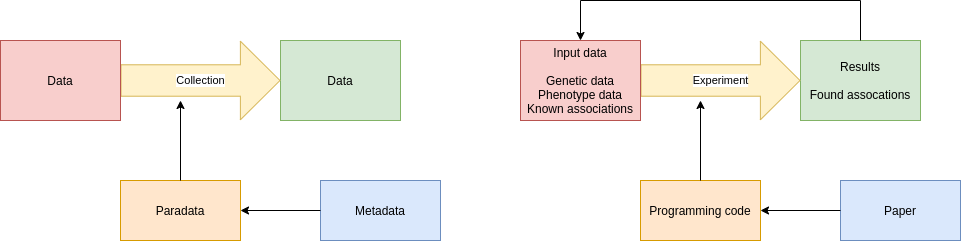
\includegraphics[width=\linewidth]{figure_1.png}
  \caption{
    Left: general relation between data, paradata and metadata.
    Middle: the same relations specified for eBird.
    Right: the same relations specified for genetic epidemiology.
  }
  \label{fig:figure_1}
\end{figure}

% \paragraph{Simple example of paradata}

A simple example would be the data at eBird (\url{https://ebird.org/}),
where people can submit wher a bird of a certain species was spotted.
The name of the person that spotted that bird is paradata, 
as it is that person that generated the data and determined of
which species the bird was, 
as shown schematically in the middle panel of Figure \ref{fig:figure_1}.

% \paragraph{Relevance of paradata}

Paradata is relevant, as it allows primary data to be re-used.
In the eBird example, it helps assess the trustworthiness of the 
data, as beginner birdwatchers tend to make more mistakes in identifying
the correct bird species, as compared to experts.
By using the name and/or experience of the birder as a covariate,
we can re-use the dataset in other contexts as well,
as now this example can be generalized to
a classification problem of unlabeled
data for learning agents with different amounts 
of experience.

% \paragraph{This paper is about computer code}

This paper is about paradata in the context of a computational
experiment in general and uses an example from genetic 
epidemiology in particular.
We'll postpone the introduction to genetic epidemiology now
and focus on 'computational experiment' first.
A computational experiment is an experiment run by computer code.
In chronologic order, it usually collects primary data first, 
then runs an analysis, which finally results in the generation of results.

This paper takes the standpoint that it is the computer code 
that describes this generation of results, 
hence it is the computer code that is paradata 
(i.e. not the description of the experiment as done in a natural language),
as shown schematically in the right panel of Figure \ref{fig:figure_1}.
Reading the computer code allows one to assess the trustworthiness 
of the experiment, similar to knowing the name or expertise of a bird spotter.
Having the code allows one to 
verify, re-use and extend the experiment, 
in the same or other contexts, providing for reproducible research.
Additionnally, this paper suggests some best practices on how to make 
an experiment FAIR data (findability, accessibility, interoperability, and reusability) \cite{wilkinson2016fair} better.

%%%%%%%%%%%%%%%%%%%%%%%%%%%%%%%%%%%%%%%%%%%%%%%%%%%%%%%%%%%%%%%%%%%%%%%%%%%%%%%%
\section{Genetic epidemiology}
%%%%%%%%%%%%%%%%%%%%%%%%%%%%%%%%%%%%%%%%%%%%%%%%%%%%%%%%%%%%%%%%%%%%%%%%%%%%%%%%

% \paragraph{Introduction}

This paper uses genetic epidemiology as a specific example,
to illustrate that the computer code is paradata,
that this paradata is relevant, as it helps 
to assess the correctness of the results,
where the correctness of the results is relevant for 
science in general and healthcare in particular.
However, any field that uses computation in its experiments
could be used as an example.

% \paragraph{For some fields, the experiment is actually run by code}

Genetic epidemiology is a field within biology that, among 
others, measures the spread of heritable traits,
as well as how these come to be.
For example, we know that lactose intolerance is, among others,
caused by producing too few lactose-degrading enzymes,
and is most commonly found in south-east asia.
The trait is caused by the genetic make-up, 
or genotype 
(see Table \ref{tab:definitions} for the definitions of terms used in this paper), 
of a person.
The trait, also called phenotype (again, see Table \ref{tab:definitions}), 
in this example is lactose intolerance,
yet any human property, such as weight or height can be studied.
Genetic epidemiology studies the spread of genotypes and phenotypes,
as well as the relation between those two.
When an association between genotype and phenotype is found,
these associations are subsequently used to 
create gene panels, where the gene causing 
an association is measured specifically, to, among others,
detect people at risk for the associated phenotype.

The rest of this section describes a genetic epidemiology study 
in more detail, with special focus on the computational experiment.

\iffalse
\begin{figure}[!htbp]
  \centering
  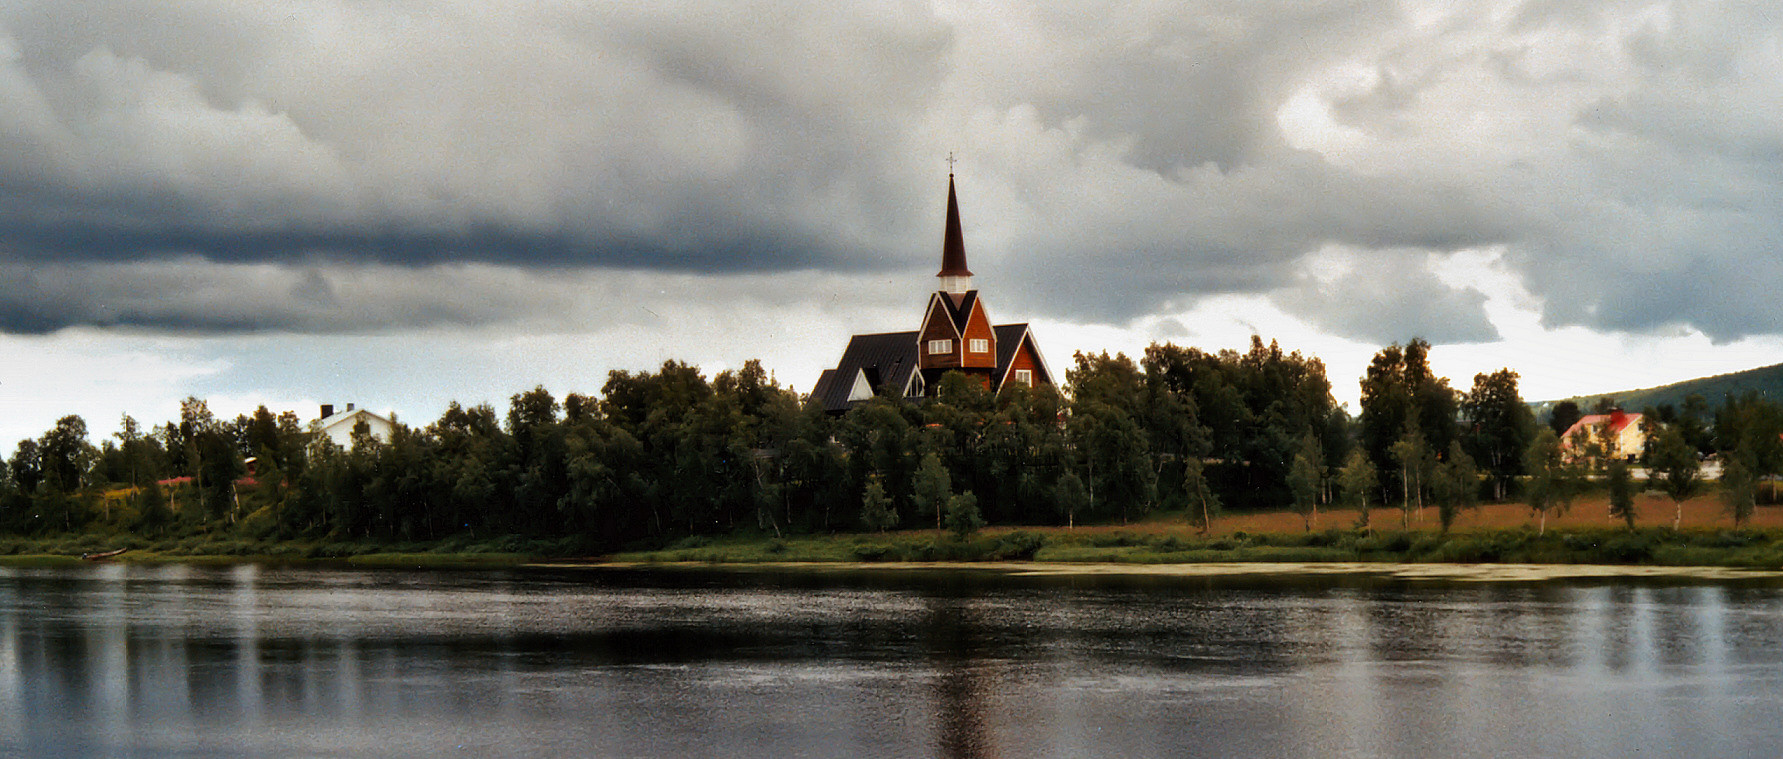
\includegraphics[width=\linewidth]{Karesuando_church.jpg}
  \caption{
    Picture of Karesuando's church,
    the village where the Northern Swedish Population
    Health Study started.
    From \cite{hopfner2005}
  }
  \label{fig:karesuando_church}
\end{figure}
\fi

The example study followed is a pseudorandomly selected paper
from \cite{ahsan2017relative}. The primary data used by that paper is
from a population study called the Northern Swedish Population
Health Study (NSPHS) that started in 2010 \cite{igl2010northern}. 
The approximately 1000 participants were initially mostly surveyed
about lifestyle \cite{igl2010northern} and follow-up studies
provided the type of data relevant for this paper, 
which are (1) the genotypes \cite{johansson2013identification},
(2) the phenotypes, which are the concentrations of certain proteins
in the blood \cite{enroth2014strong,enroth2015effect}.

\iffalse
\begin{figure}[!htbp]
  \centering
  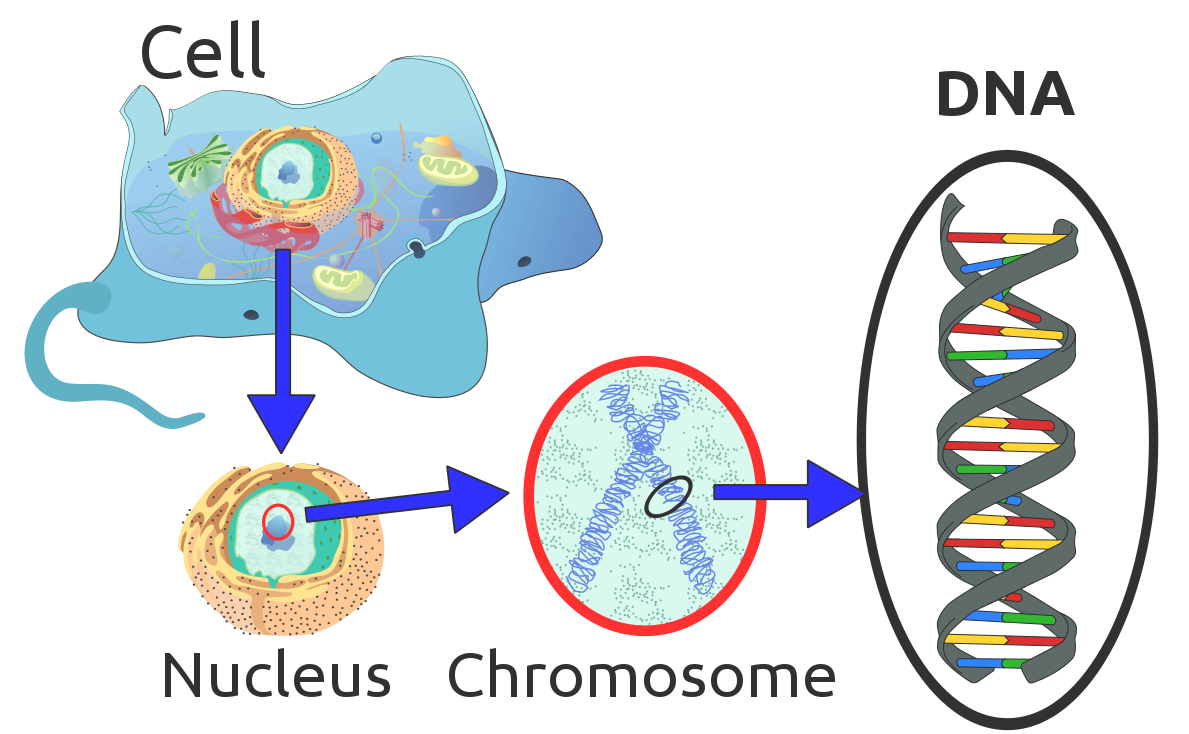
\includegraphics[width=\linewidth]{1189px-Eukaryote_DNA-en.png}
  \caption{
    A cell has a nucleus that contains chromosomes. 
    Each of these chromosomes (46 in humans) consist out of DNA. 
    DNA itself conists out of 4 nucleotides, 
    as depicted by the horizontal sticks 
    with the colors red, yellow, green and blue.
    From \cite{sponk2012}
  }
  \label{fig:eukakyote_dna}
\end{figure}
\fi

The first type of primary data, the genotypes, 
consists out of single nucleotide polymorphisms (SNPs, pronounced as 'snips').
A SNP has a name and a location on the DNA, at which there is a certain nucleotide.
DNA (organized into chromosomes and present in every (nucleated) cell, 
see figure \ref{fig:eukakyote_dna}) 
consists out of billions of nucleotides.
There are four types of nucleotides, 
called adenosine, cytosine, guanine and thyrosine, all commonly abreviated
as A, C, G and T respectively.
One SNP example is \verb|rs12133641|, which is a SNP located at position 
154,428,283, where 67 percent of the people within this study have an A,
and 33 percent have a G (also from \cite{ahsan2017relative}, Table S3).

\iffalse
\begin{figure}[!htbp]
  \centering
  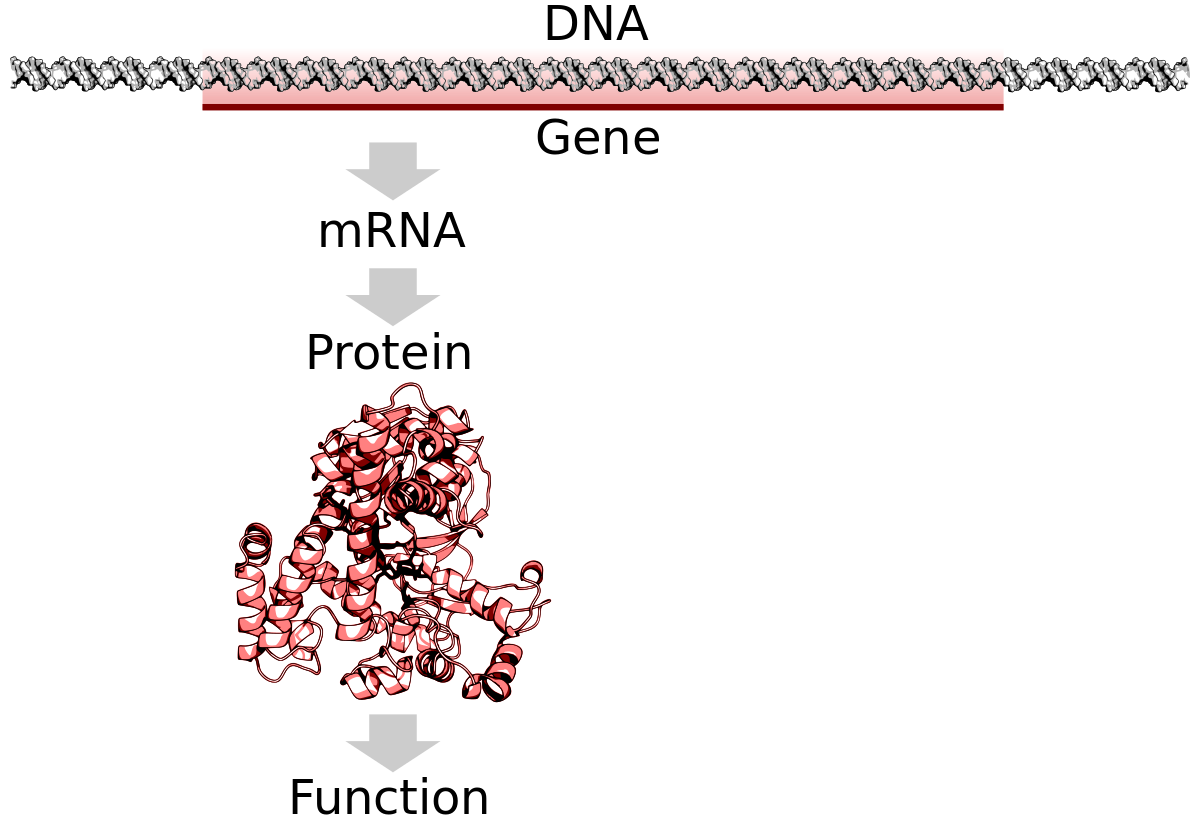
\includegraphics[width=\linewidth]{DNA_to_protein.png}
  \caption{
    Parts of DNA (so-called 'genes') code for proteins. 
    The DNA, that always stays put in the cell's nucleus, 
    is transcripted to messenger RNA (mRNA).
    mRNA leaves the nucleus and its code gets translated to 
    a protein sequence.
    Near the start of a gene are regions that determine the amount
    of proteins produced (not shown in figure).
    Adapted from \cite{shafee2015}
  }
  \label{fig:dna_to_protein}
\end{figure}
\fi

The second type of data, the phenotypes, 
are concentrations of proteins in the blood. 
DNA contains the code for building proteins (see Figure 
\ref{fig:dna_to_protein}), 
as well as the rate
at which a protein is created. Some proteins end up in the blood and
their presence can be used to assess the health of an individual.
IL6RA is one such protein and, spoiler alert, its concentration
is associated with the SNP mentioned earlier.

The field of genetic epidemiology looks -among others- for
correlations between genetic data and biological traits.
For example, figure \ref{fig:ahsan2017relative_table_2_sub} 
(from \cite{ahsan2017relative}) shows that
SNP \verb|rs12133641| is highly correlated (p-value is $3.0^{-73}$, 
for $n$ = 961 individuals) with protein IL6RA. What this results does
not yet teach us, is how this correlation works, yet
figure \ref{fig:ahsan2017relative_s6} shows us the direction of the association:
the X axis shows the possible genetic make-ups (aka the genotype) of the individuals,
where 0 denotes the individuals with genotype
AA (the individual inherited one adenosine 
from his/here mother and one adenosine from his/her father), 
1.0 denotes AG (one A is inherited from one parent, 
where the G is inherited from the other parent) and 2.0 denotes GG.
From Figure \ref{fig:ahsan2017relative_s6} we can conclude that, on average,
the more guanines are present at that SNPs location,
the higher concentration of IL6RA can be found in a human's blood.

The amount of variance that can be explained by an association (i.e.
the R squared value) is rarely 100 percent, which means that a trait (in
this case, the concentration of IL6RA) cannot be perfectly explained
from the genotype alone. As we can see in figure \ref{fig:ahsan2017relative_s6}, 
43 percent of the variance can be attributed to an individuals'
genotype. 
Additional factors, 
such as the effect
of the environment (e.g. geographic location, time of day), 
lifestyle (e.g. smoking yes/no) or having a disease (e.g. diabetes) 
are needed to explain the additional variation.

\iffalse
\begin{figure}[!htbp]
  \centering
  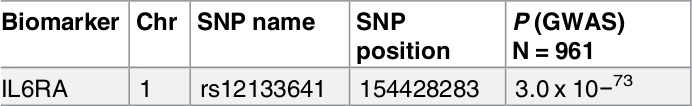
\includegraphics[width=\linewidth]{ahsan2017relative_table_2_sub.png}
  \caption{
    An example result of a genetic epideological research.
    It shows that the SNP named rs12133641 (located at position 154,428,283
    of chromosome 1) is highly correlated (p value is 3.0 * 10e-73, 
    961 individuals) to the concentration of the protein IL6RA, as measured
    in blood. The table is a simplified result from \cite{ahsan2017relative}.
  }
  \label{fig:ahsan2017relative_table_2_sub}
\end{figure}
\fi

\iffalse
\begin{figure}[!htbp]
  \centering
  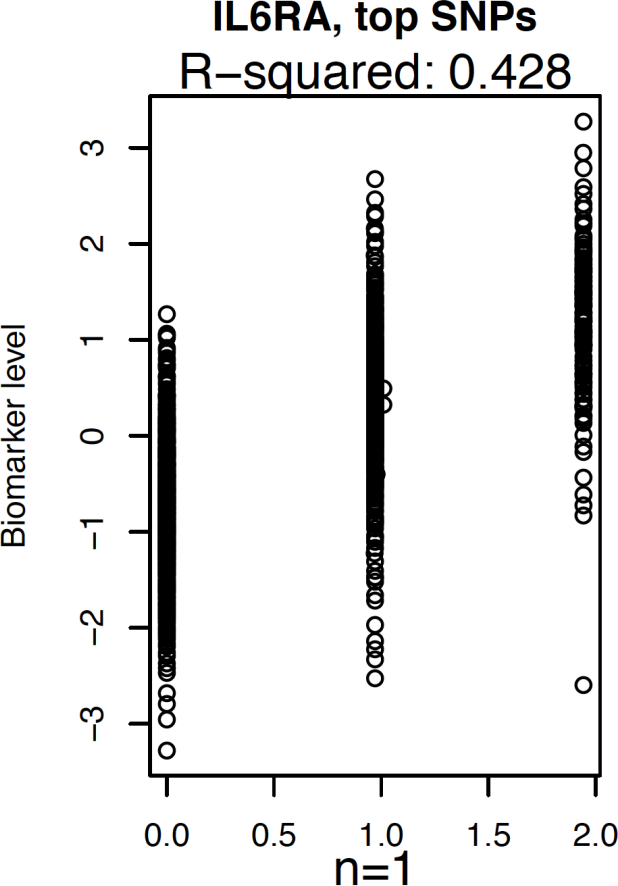
\includegraphics[width=\linewidth]{ahsan2017relative_s6.png}
  \caption{
    The relation between the genotype for SNP rs12133641 
    and the protein concentration of IL6RA is relatively strong.
    The X axis shows the the genotype of the individuals,
    where 0 denotes AA, 1.0 denotes AG and 2.0 denotes GG.
    The Y axis shows the concentration of the protein IL6RA 
    as found in the participants' blood. n = 1 denotes the number
    of SNPs that were determined to be involved.
  }
  \label{fig:ahsan2017relative_s6}
\end{figure}
\fi

These conclusions may end up in the clinic.
For the sake of having a clear example,
let's assume that a high level of IL6RA 
is associated with a disease that develops later in life,
yet is preventable by lifestyle changes.
Would this be the case, we can create a gene panel that specifically measures
SNP \verb|rs12133641|. 
If the gene panel shows an individual has two guanines, 
we know that this person is likelier to develop higher levels of
IL6RA and is likelier to benefit from the lifestyle changes.

In this simple example, it will be easier
to measure the level of IL6RA in the blood, than using a gene panel.
However, there are associations published for many diseases,
in which multiple SNPs contribute to being more likely 
to develope a disease in the future. Here, the phenotype (having 
a disease in the future) is impossible to detect at the present
and associations found in earlier studies are used to create a gene panel.
As creating a gene panel is costly, those associations better be correct.

%%%%%%%%%%%%%%%%%%%%%%%%%%%%%%%%%%%%%%%%%%%%%%%%%%%%%%%%%%%%%%%%%%%%%%%%%%%%%%%%
\section{Code is more important than the paper}
%%%%%%%%%%%%%%%%%%%%%%%%%%%%%%%%%%%%%%%%%%%%%%%%%%%%%%%%%%%%%%%%%%%%%%%%%%%%%%%%

% \paragraph{The experiments within genetic epidemology works are done by code}

The experiment described above is run by code. 
It was code that detected the relationship between the genotype
(in this case, SNP \verb|rs12133641|) 
and the phenotype (in this case,the concentration of IL6RA).
To detect this association, 
there was no fieldwork, nor lab-work involved.
For this experiment, 
it has been the researcher that has written the code,
after which that code does the actual work. 
A genetic epidemiologist does not need a lab, but computational power instead.

To \emph{obtain} the raw genetic data, yes, there may be fieldwork and/or lab-work
involved. For example, a researcher needs to go into the field to take
samples (e.g. blood) of humans or other species. To analyse these samples,
a researcher needs a lab. Depending on the technique being used on
how to analyse the samples, there may be a big bioinformatics step
to aggregate the measurements into useful genetic data. 
Although this paper does not focus on the code run to 
aggragate the raw data into useful genetic data, the same arguments
can be made for that code as in the example: that code is 
the ground truth of how the raw data is collected into useful genetic data.

% \paragraph{The code is the paradata for the results of an experiment}

Programming code (from now on: 'code') is paradata, 
as it is data that describes how data is generated.
Code is data that is usually in the form of text, 
spread over one or more files, that describes the experiment.
The computational experiment (from now on: 'experiment') collects the data
and then looks for patterns.
Those patterns (again, a type of data) are the results of an experiment.

The (scientific) article is metadata, as it is data that describes other data:
an article describes the
experiment (and hence the programming
code) in a natural language, which is usually English (at this point in time). 
However, a natural language is not the best
candidate to describe how the data is collected,
as it has a loose connection with collecting the data.
If the code and article of an experiment disagree,
it is the code that actually let the data be collected.  
Instead, an article is metadata about a research.

% \paragraph{Science should be reproducible}

A scientific claim must be reproducible before it is accepted
by the scientific community.
Reproducibility (i.e. to reproduce the same results) 
and replicability (i.e. to reconclude a conclusion)
are fundamental characteristics of scientific studies \cite{patil2019visual}.
For computational science, it is relatively easy to 
reproduce an experiment, as all it takes is a computer, electricity,
an optional internet connection, the code and the data.
In computational science, however, it appears that 
culture to reproduce results has been lost 
and to counter this, it has been suggested to make
reproducible research a minimal requirement for 
publication \cite{peng2011reproducible}.

% \paragraph{Code should be published}

\iffalse
\begin{figure}[!htbp]
  \centering
  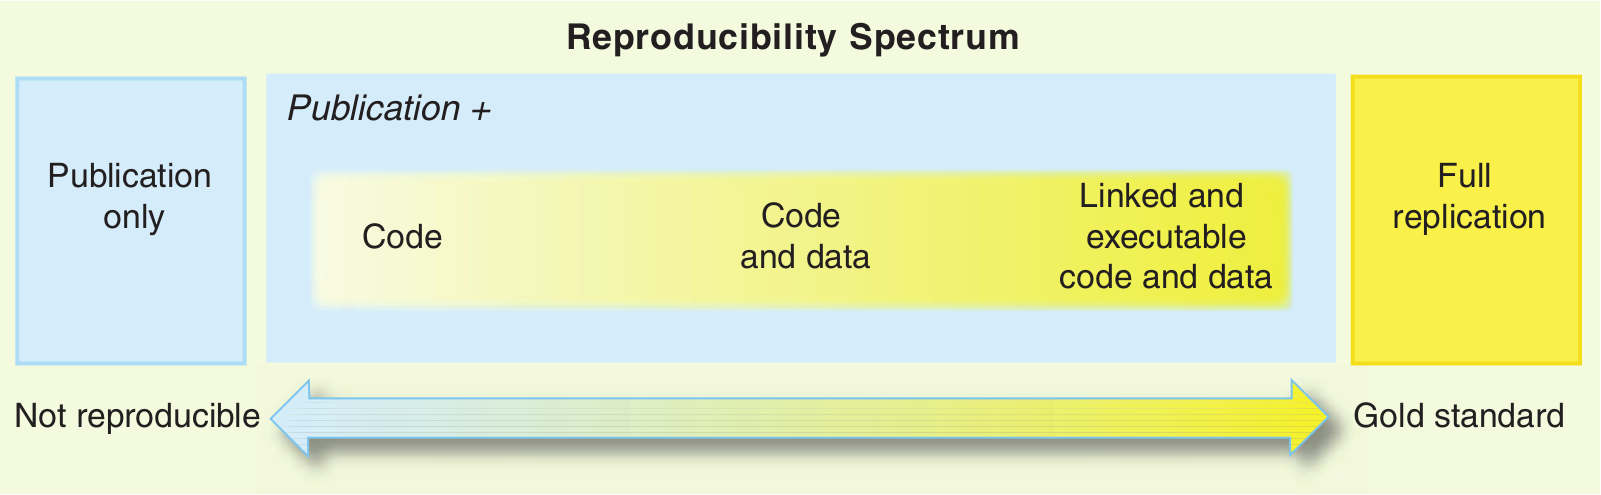
\includegraphics[width=\linewidth]{peng2011reproducible_fig_1.png}
  \caption{
    Levels of reproducibility, from \cite{peng2011reproducible}
  }
  \label{fig:peng2011reproducible}
\end{figure}
\fi

The code of a computational experiment must be published
for an experiment to reproducible.
It is however (too) common that the original data
and/or code are unavailable \cite{peng2021reproducible}.
One saddening example is described in \cite{haibe2020importance}, where
an algorithm that detects breast cancer better than a human expert,
was irreproducible.
In the case of genetic epidemiology, it is a given that the original
data cannot be published as this data is sensitive.
The code of a computational experiment, however, \emph{can} be
distributed without such problems.
It is, however, not code that is published, but an English
description of what that code does instead.
From a knowledge management's perspective,
to conserve an experiment,
it is the code that must be archived and not the
English description of what it does:
it is the code does the actual work.
Hence, from a knowledge management perspective, emphasis should be
put more on the preservation of code, as it is the most important actor
in an experiment.

% \paragraph{Example of code being the ground truth}

Code should be published, as it holds the
ground truth of an experiment; it does the actual work.
The more complex the computation pipeline is, the easier it is
to have a mismatch between the article (that describes what the
code does) and the code (that actually does the work).
It is easy (tempting?) to overlook how easy it is to have a mismatch
between paper and code.

To illustrate how easy it is to get a mismatch between a paper
and the code, consider this fictional example
of a text in a paper:

\begin{verbatim}
We compared the values of x and y using a one-tailed Student's T-test,
as we expect the average value of x to be less than the average value of y.
\end{verbatim}

We ignore the choices of words and style of this sentence: what is
important is the content: a one-tailed T test is performed.
Taking a look at the (in this case, the programming language R) code, 
we find the following line:

\begin{verbatim}
t.test(x, y)
\end{verbatim}

The line of code is simplified (as the result of the T test is never stored),
but the code is correct:
\verb|t.test| is indeed the name of an R function to do a T-test
and it is reasonable to assume that this code, when found in the code
of an article, is correct.

Here, however, we see a mismatch between the English description and the code:
by default, the R function \verb|t.test| does a \textbf{two}-tailed T-test.
A consequence of this fictional example is that the published p-values are
higher than needed, resulting in less significant findings, which
results in (needlessly) less conclusions drawn from a paper.

\iffalse
\begin{figure}[!htbp]
  \centering
  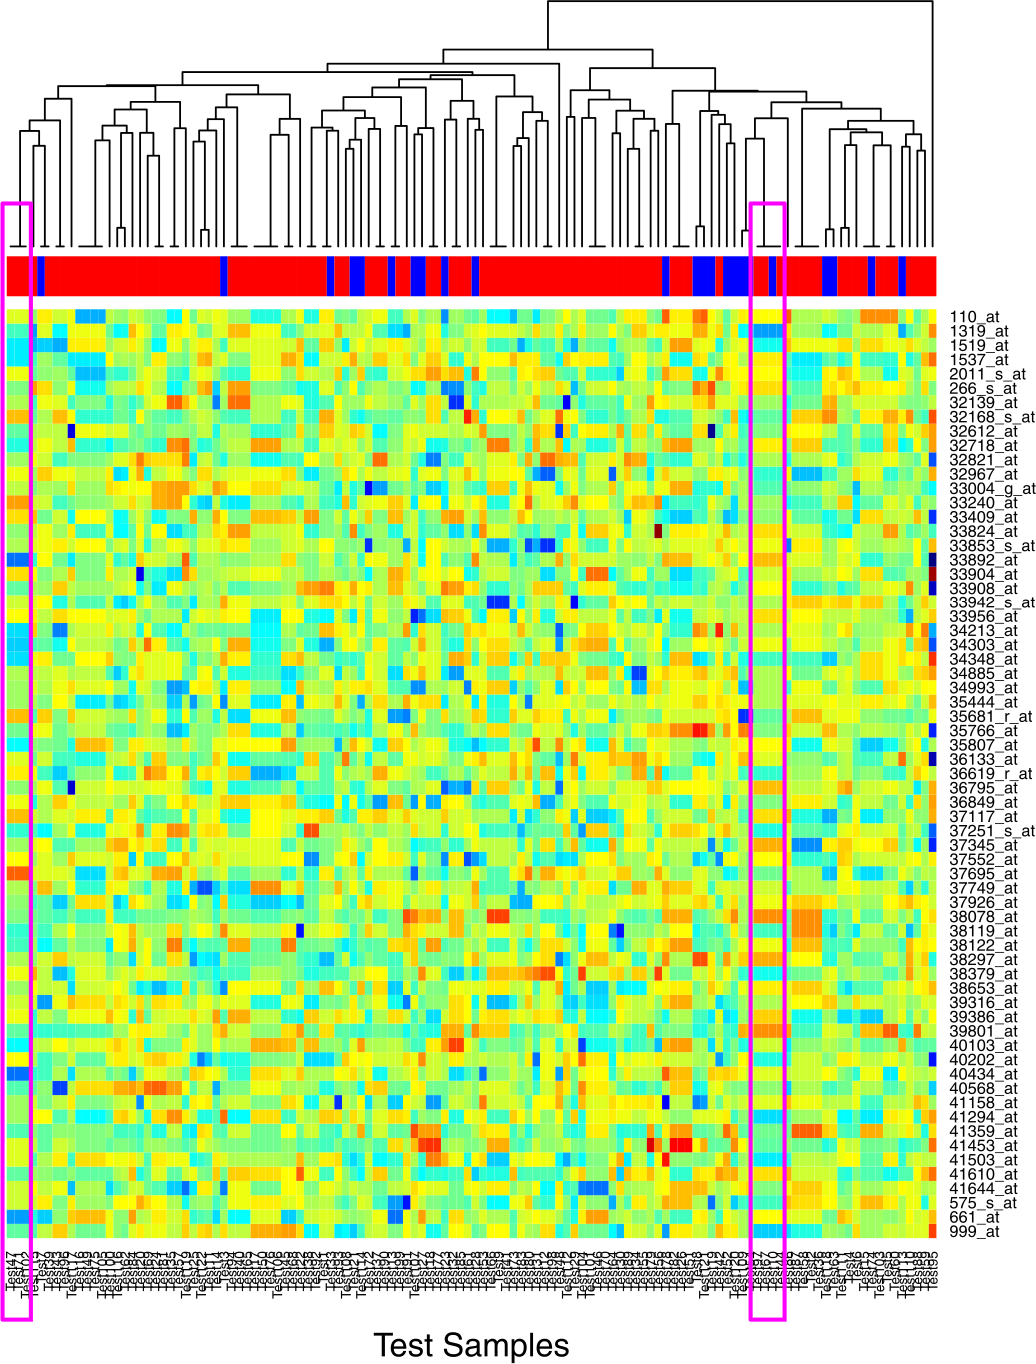
\includegraphics[width=\linewidth]{baggerly2009deriving_fig_1a.png}
  \caption{
    Gene expression result due to an off-by-one error.
    The cells in the main table show how much mRNA is produced per cell 
    line (the columns) for different proteins (the rows).
    The colors above the cells, with the dendrogram, shows
    red for cells that do not respond (red) and do respond (blue) to an 
    antibiotic.
    The purple rectangles show samples that are duplicated.
    Note that, due to this, some
    samples that behave identically are both non-responders and responders.
    From \cite{baggerly2009deriving}
  }
  \label{fig:baggerly2009deriving}
\end{figure}
\fi

One pseudorandom example of a mismatch between code and article
was found by me in \cite{labrecque2019interpretation}.
After the corresponding author of that paper was contacted,
the code was updated and confirmed to have the same
results as published in the paper.

It is the paper that accompanies the code,
as it is the code that generates the results.
When humans are fallible and code gets bigger, the likelihood of
a mismatch between the English paper and the code increases.
We know that the most common errors are 
simple (and may legitimately fear that those simple errors are common) 
\cite{baggerly2009deriving},
and this example is not too far off from the
examples given in that paper.

But regardless of the size of the code, 
it is the code that is the ground truth.

%%%%%%%%%%%%%%%%%%%%%%%%%%%%%%%%%%%%%%%%%%%%%%%%%%%%%%%%%%%%%%%%%%%%%%%%%%%%%%%%
\section{There are multiple way to publish code}
%%%%%%%%%%%%%%%%%%%%%%%%%%%%%%%%%%%%%%%%%%%%%%%%%%%%%%%%%%%%%%%%%%%%%%%%%%%%%%%%

As it is the code that is the most important actor in an the experiment,
it should be treated as equally or more important than the scientific
paper describing what is does.
Regardless of this, most academic journals, 
when concerning computational experiments
only review the (usually) English description of the code
and make the review of code optional.
One notable exception is rOpenSci \cite{ram2018community},
which is an organisation that does peer-review academic code 
and facilitates the optional publication of a paper.
Although both code and paper are peer-reviewed,
most effort is spent on reviewing the code,
as can be seen in, for example, 
the \verb|mcbette| R package \cite{bilderbeek2020mcbette}.

There are multiple ways of publishing code,
that require increasingly more knowledge to do and result
in increasingly more reproducible experiments:
(1) publishing the code as text only, e.g. by printing
it in a Supplementary Materials, (2) publishing
the code on a hosted website, e.g on GitHub, with
added features (3) publishing 
the installed code within a virtual environment,
for example, using a Singularity container.
Here I will go into details of each of these ways.

%%%%%%%%%%%%%%%%%%%%%%%%%%%%%%%%%%%%%%%%%%%%%%%%%%%%%%%%%%%%%%%%%%%%%%%%%%%%%%%%
\subsection{Publishing raw code}
%%%%%%%%%%%%%%%%%%%%%%%%%%%%%%%%%%%%%%%%%%%%%%%%%%%%%%%%%%%%%%%%%%%%%%%%%%%%%%%%

Code is commonly published alongside of a 
paper, pasted as text in the Supplementary Materials 
(for example, in \cite{labrecque2019interpretation}).
This is the rawest form of publishing code,
as it is just text.

% \paragraph{Raw code is important}

The raw code of a computational experiment is
more important to preserve than the article describing
the experiment, even when both describe the experiment identically,
correctly and reproducibly, 
as it has/should been that code that generated the results of an experiment.
Again: if the paper and code differ, it is the code that did
the actual work with the actual/true results.

% \paragraph{Raw code is an indicator of quality}

Raw code gives an indication of the quality 
of a computational experiment and several metrics are
devised to get an idea of the quality of code.

The simplest metric to assess the quality of code is 
the amount of (single) lines of code (SLOC). 
Code that has a lower SLOC count, i.e. it is more concise,
is usually regarded as having a lower chance of containing bugs.
Additionally, following a style guide (e.g. \cite{style_guide}), 
improves software quality \cite{fang2001}.

A more interesting metric is the cyclomatic complexity of the code.
The cyclomatic complexity is defined as the number of ways that
the code can be executed. 
For example, code that has only one \verb|if| statement
has a cyclomatic complexity of 2, as the condition within the \verb|if|
statement can be true or false.
The cyclomatic complexity correlates with code complexity,
where more complex code is likelier to contain or give rise to bugs 
\cite{abd2018calculating,chen2019empirical,zimmermann2008predicting}

A feature that deserves more attention
is that 'code must act as a teacher for future developers' \cite{sadowski2018modern}.
Error handling is one of the mechanisms to do so.
A simple example is when one (e.g. a BSc student) 
needs to calculate the variance of a distribution.
Commonly one needs to call a function to do so, 
e.g. \verb|var| in R, that needs the values of the distribution
as input.
However, to calculate the variance of a distribution, at least two values
are required. 
When the variance of (zero or) only one value is requested,
an error message can helpfully indicate that the function 
needs at least two values.

% \paragraph{The problems with raw code}

There are multiple problems with publishing raw code.
First, there is no guarantee that that code \emph{can} actually
run, for example, due to a typo added after the code was pasted.
Secondly, there is no way to determine if code that worked yesterday
works today. These problems can be prevented by, instead of
pasting raw code, using a website to host that code (see below).

% \paragraph{Raw code is already better than no code}

Publishing raw code is already better than not publishing code at all,
as that raw code can be assumed to have run successfully at least once.
To reproduce an experiment from raw code can be painful, 
yet it is usually better than writing the same code from scratch.

%%%%%%%%%%%%%%%%%%%%%%%%%%%%%%%%%%%%%%%%%%%%%%%%%%%%%%%%%%%%%%%%%%%%%%%%%%%%%%%%
\subsection{Publishing hosted code}
%%%%%%%%%%%%%%%%%%%%%%%%%%%%%%%%%%%%%%%%%%%%%%%%%%%%%%%%%%%%%%%%%%%%%%%%%%%%%%%%

Code is sometimes published alongside a paper, 
in the form of a hosted website.
This way of publishing code gives additional options,
both for the authors of that code, as well as its users.
This practice has increased,
with the abstracts from articles in the academic journal
'Bioinformatics' referring to such a hosted website
has increased tenfold, going from below 5 percent in 2009 
to around 50 percent in 2017 \cite{russell2018large}.

% \paragraph{Example of hosted code}

There are multiple websites for hosting code, with BitBucket, GitHub,
GitLab and SourceForge being the most well-known.
GitHub is currenly the most popular website to host code in general,
with millions of users.
GitHub users can create dedicated websites (called 'repositories')
to upload code. Code hosts, such as GitHub, 
store that uploaded code and provide ways 
for visiters to download the code and/or interact with it.
The use of such code hosting websites
accommodates collaboration \cite{perez2016ten}.
and improves transparency \cite{gorgolewski2016practical}.
An example from the author is the website \cite{bbbqarticleissue157},
that hosts part of the code for the paper \cite{bilderbeek2022transmembrane},
as shown in Figure \ref{fig:bbbqarticleissue157}.

\iffalse
\begin{figure}[!htbp]
  \centering
  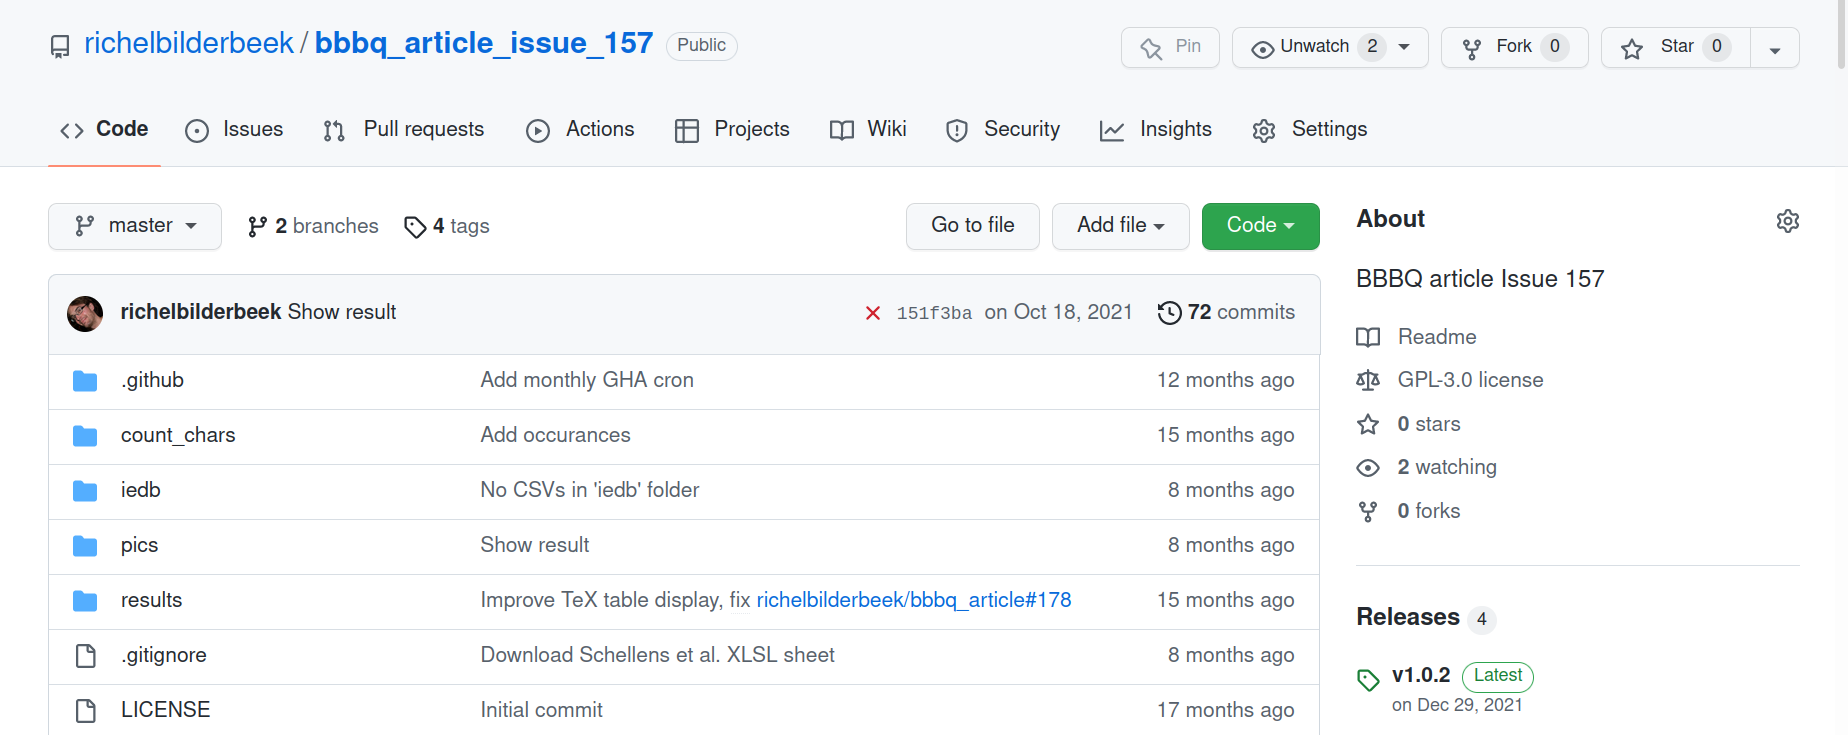
\includegraphics[width=\linewidth]{bbbq_article_issue_157.png}
  \caption{
    A typical GitHub repository \cite{bbbqarticleissue157}, 
    hosting the code for a
    computational experiment, 
    as published with \cite{bilderbeek2022transmembrane}.
    Note that this repository has 72 commits, where a commit is a change
    to the code.
  }
  \label{fig:bbbqarticleissue157}
\end{figure}
\fi

% \paragraph{Hosted code has important metadata}

Hosted code has many additional features, such as
a version-controlled history, continuous integration scripts
and automatically generated metrics.
A code hosting website produces and shares this metadata.
This metadata can help to determine the
reproducibility, correctness and quality of code
of computational experiments.

% \paragraph{Hosted code has a commit history}

Hosted code commonly has a commit history. For example, GitHub
uses a version control system called \verb|git| (hence its name).
In practice, this means that when a change is made to the code,
a new version is created. In the case that the change was harmful,
one can go back to an earlier version and continue again from there.
It is a general recommendation to put version control
on all human-produced data \cite{wilson2014best}.

% \paragraph{A commit history helps assess honest reporting}

Hosted code improves transparency \cite{gorgolewski2016practical}.
The history of changes, called the commit history, 
helps to assess the honesty in the reporting of the code. 
Ideally, the full version history of the code 
has been generated, by hosting the code directly at its inception.
However, in some repositories, only the final version of the code has been
posted, which means all historical information is lost.
From a code history, it can be observed, for example, 
how much statistical tests have really/actually been done 
and see if all are reported:
failing to reporting a (usually non-significant) statistical tests is 
one of the many degrees of freedom 
in p-value hacking \cite{wicherts2016degrees}.

% \paragraph{Continuous integration helps assess code quality}

Some code hosts, among others, GitHub, 
allows the researcher to start software scripts when uploading a new version.
To determine the reproducibility of the code, one such script should
run the code (on trivial data) to verify if the code works at all.
If the functionality of the code is lost, the researcher
can immediatly see which small change was the cause of this.
A formalized version of this workflow is called continuous integration (CI).
Using a CI service (such as GitHub Actions), is known to significantly 
increase the number of bugs exposed \cite{vasilescu2015} and increases
the speed at which new features are added \cite{vasilescu2015}.
Using CI opens up the possibility to informally annotate features of
a repository. For example, Figure \ref{fig:build_badge} shows a 
build badge that indicates that a LaTeX document (i.e. this paper)
could be built.

\iffalse
\begin{figure}[!htbp]
  \centering
  
\includegraphics[width=\linewidth]{build_badge.png}
  \caption{
    A build badge for the GitHub repository of this article.
    The description indicates which process it is that the badge
    signals success (as in this case) or failure of. 
  }
  \label{fig:build_badge}
\end{figure}
\fi

% \paragraph{Code coverage helps assess code quality}

Testing, in general, is an important mechanism to ensure
the correctness of code (an interesting example is \cite{rahman2020exploratory}
showing bugs in scientific software on the COVID-19 pandemic. 
It recommends more testing).
The percentage of (lines of) code tested is called the code coverage.
Code coverage correlates with code quality \cite{horgan1994,del1995correlation}. 
The non-profit organisation rOpenSci \cite{ram2018community},
which peer-reviews code,
has made it a prerequisite to have a code coverage of 100\%.
Also here, CI opens up the possibility to informally annotate the
code coverage. For example, Figure \ref{fig:badge_codecov} shows a 
build badge that indicates that certain R package's code 
has a 100\% code coverage.
Hence, code coverage is important metadata, that can automatically
be acquired when using code hosting website.

\iffalse
\begin{figure}[!htbp]
  \centering
  
\includegraphics[]{badge_codecov.png}
  \caption{
    A build badge for the code coverage of an R 
    package (\url{https://github.com/ropensci/beautier}).
    The umbrella signals that the code coverage is hosted by
    CodeCov (\url{https://codecov.io/}). 
    The text indicates which process it is that the badge
    signals, which in this case, is that the code is fully covered
    by tests.
  }
  \label{fig:badge_codecov}
\end{figure}
\fi

% \paragraph{Metrics help assess the honest division of labour}

Most code hosts, among others, GitHub and GitLab,
automatically keep track of certain metrics.
One such metric is the amount of code each contributor has made.
In that way, authors involved in the writing of the software
are honestly acknowledged. Figure \ref{fig:daisie_contributors}
shows the number of commits the authors of DAISIE \cite{etienne2020daisie}
have made to its code.
The distribution of contributed code per author 
is useful metadata, that can automatically
be acquired when using code hosting website.

\iffalse
\begin{figure}[!htbp]
  \centering
  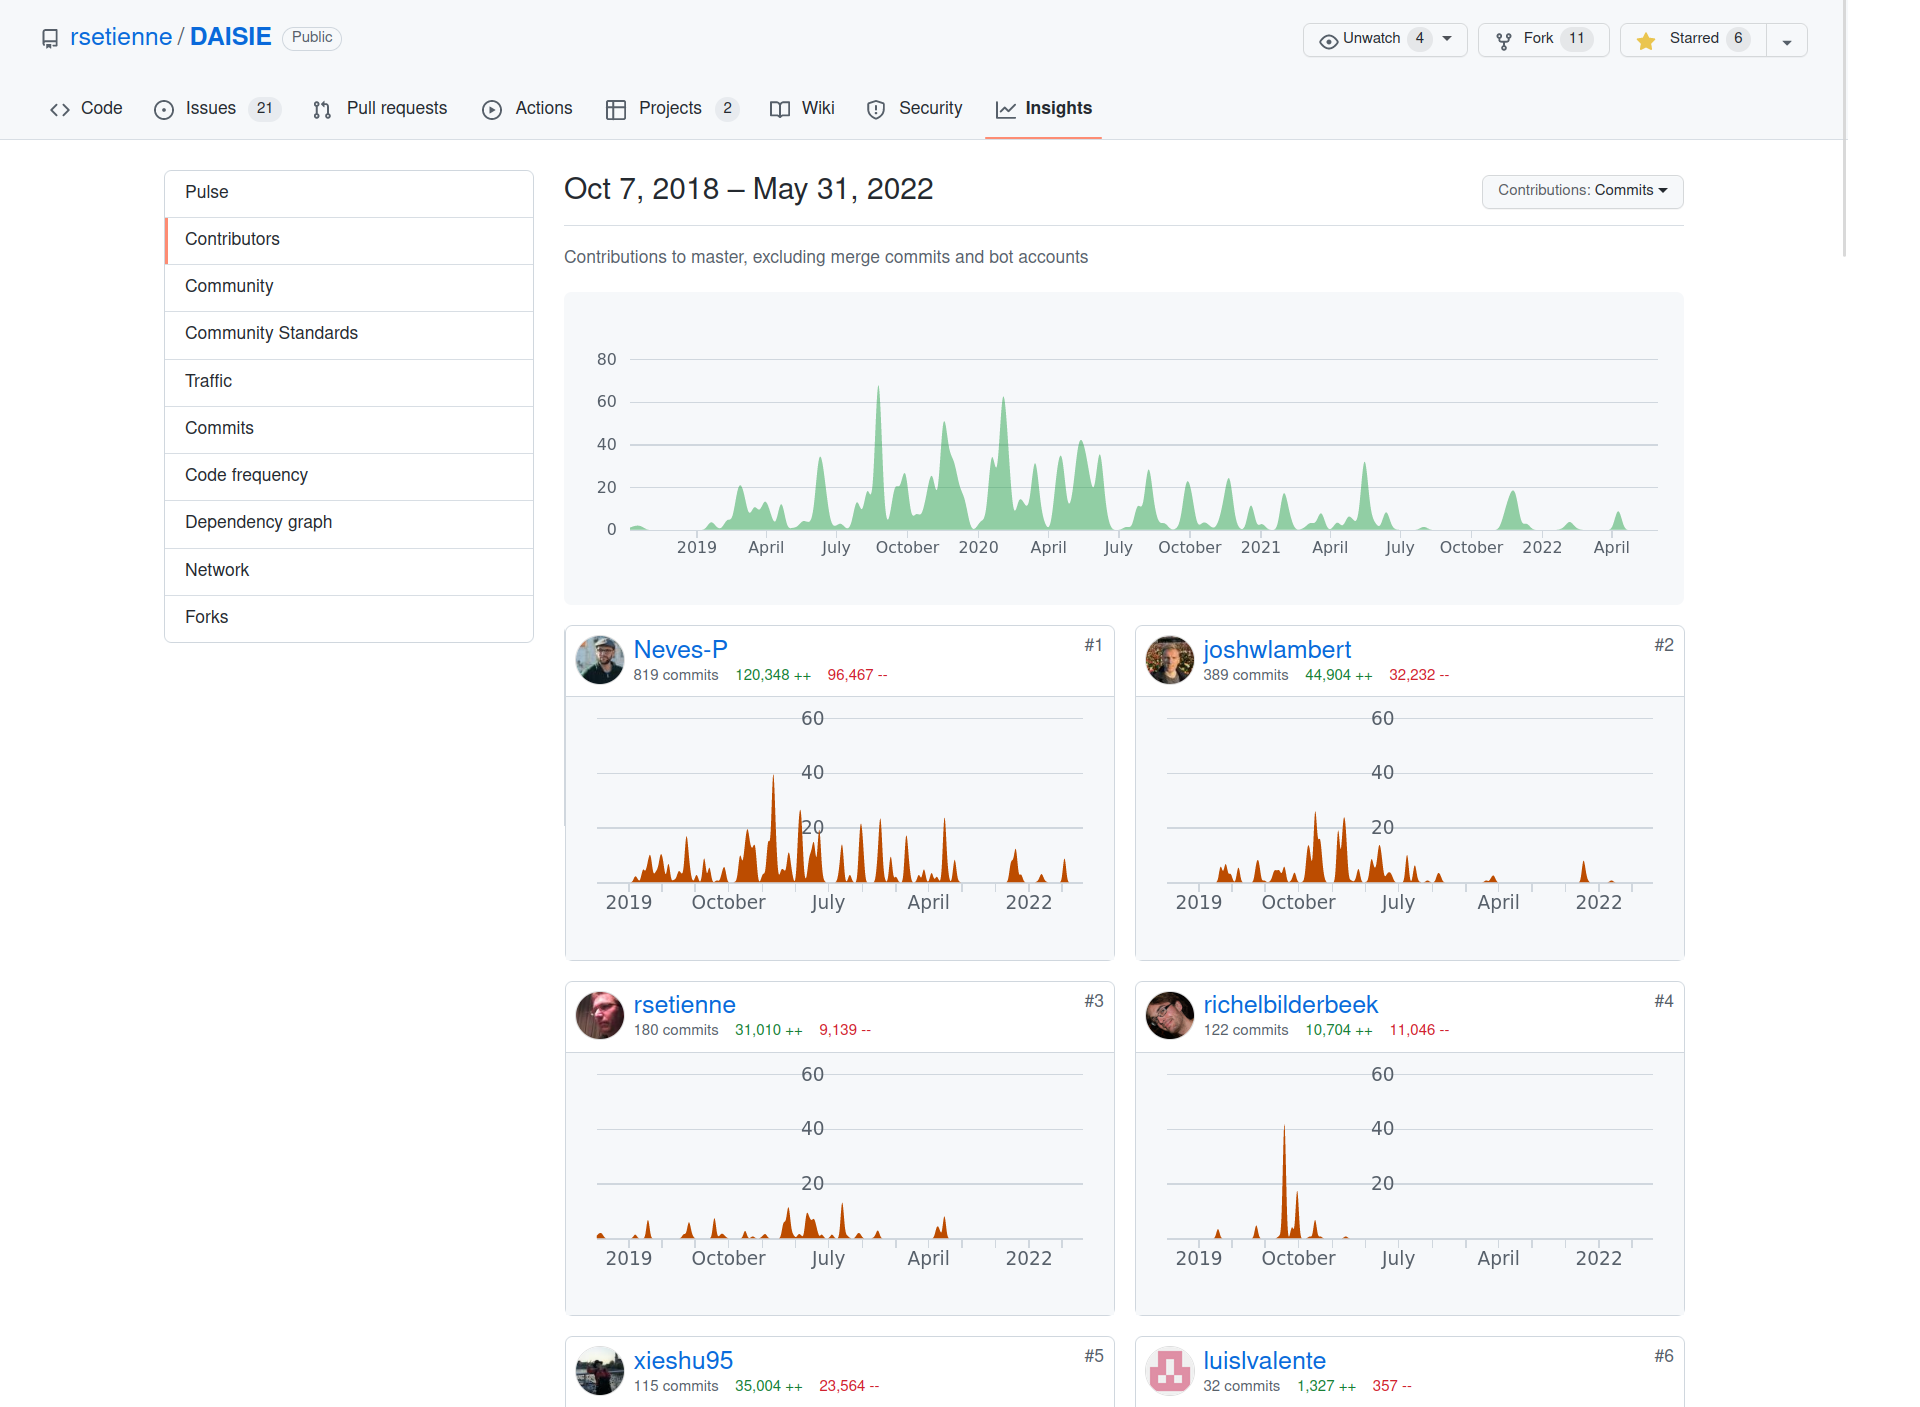
\includegraphics[width=\linewidth]{daisie_contributors.png}
  \caption{
    An overview of the commits that multiple contributors have
    made, in this case, to the code of DAISIE \cite{etienne2020daisie}
  }
  \label{fig:daisie_contributors}
\end{figure}
\fi

% \paragraph{A reader can contact the author}

A feature that gets too few attention is that code hosts
allow users to post bug reports and/or ask questions.
This allows other researchers to assess the health
of the code.
A healthy project has few open bug reports
and these bug reports should be closed within reasonable time.
When bug reports start to accumulate, this
signals either that the code contained many bugs or that
the developers lost interest in maintaining that code.
The amount of bug reports is useful metadata, 
especially when deciding to use (and depend) on a piece of software.

\iffalse
\begin{figure}[!htbp]
  \centering
  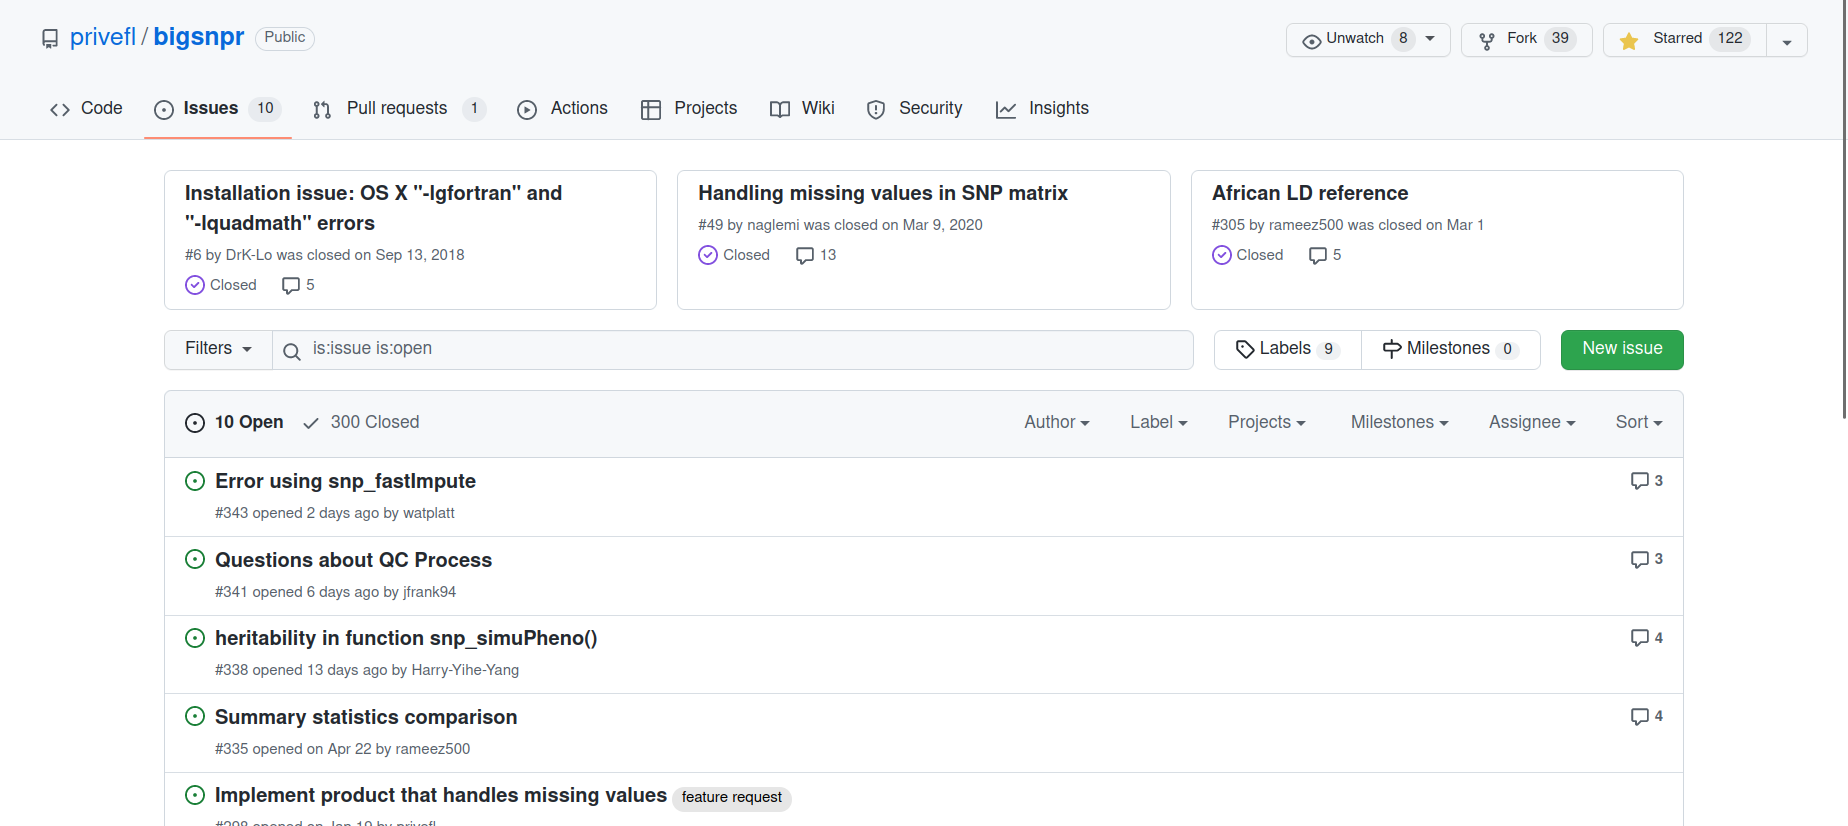
\includegraphics[width=\linewidth]{issue_ldpred2.png}
  \caption{
    An overview of the issues for the code for
    LDpred2 \cite{prive2020ldpred2}. Of the 310 issues, 300 have been closed.
    The first four issues have been replied to, as indicated by the
    talk balloon. The fifth issues has a label with the text 'feature request'
    to signal the issue type.
  }
  \label{fig:issue_ldpred2}
\end{figure}
\fi

% \paragraph{The problems with hosted code}

Albeit hosted code is vastly superior over raw code
in case of reproduciblity and correctness,
there are some problems with hosted code as well.
The most important one is that hosted code needs maintanance:
the libraries that are used by an experiment
will change over time, inevitably causing the experiment to fail
over time. 
The degradation of software is a known feature for nearly 
four decades (see the definition of 'bit rot' at \cite{steele1983hacker}),
here I will use the more modern (and in this context superior)
definition of software collapse \cite{hinsen2019dealing},
in which software fails due to dependencies on other 
software.
Where this paper recommends using older software foundations 
with multiple implementations \cite{hinsen2019dealing},
there is a modern solution that potentially has more longevity:
to publish the code installed in a virtual environment
(including the dependencies used at that time), as described below.

There is another problem that authors of academic code face,
which is that they will be contacted with a user sending in a bug report.
One solution for the author is to ignore such emails
and it can be argued that no energy should be wasted on published code
and work on something new instead.
However, upon the find of a new bug, the question is:
does all the research that use that software still 
result in the same conclusions?
A code hosting website usually has a place to report bugs
that offer transparency in the handling of bug reports.

% \paragraph{Suggestions for knowledge management}

Here are multiple suggestions to make hosted code FAIR.
To make the hosted code findable, commonly a paper refers to its URL.
At the homepage of hosted code (e.g. a GitHub repository), 
there is no standardized metadata, to,
for example, link to the paper.
Using a popular code host ensures the code is easily accessible.
There is some interoperabily supplied by a version control manager,
such as in obtaining the history of the code.
The reusability of code is reasonably easy to assess, 
by using so-called build badges.
However, there is no guarantee that a build badge that claimes success,
actually is an honest signal (i.e. that code may not actually build),
nor are there standards for what 'success' entails.

%%%%%%%%%%%%%%%%%%%%%%%%%%%%%%%%%%%%%%%%%%%%%%%%%%%%%%%%%%%%%%%%%%%%%%%%%%%%%%%%
\subsection{Publishing a virtual environment}
%%%%%%%%%%%%%%%%%%%%%%%%%%%%%%%%%%%%%%%%%%%%%%%%%%%%%%%%%%%%%%%%%%%%%%%%%%%%%%%%

The most reproducible way of submitting the code of an experiment,
is by providing the code with its dependencies installed in a virtual container.
This is close to the golden standard suggested by 
\cite{peng2011reproducible} (see also Figure \ref{fig:peng2011reproducible}),
however, that was before virtualization existed.
Virtualization allows one to provide a standard environment,
that can be used on any other computer.
The best known examples of container software are Docker and Singularity,
where the latter is the only viable option to be able to run
an experiment on a high performance computing (HPC) environment,
such as a computer cluster.

% \paragraph{Containers allow for runnable code, for longer periods of time}

Unlike English, code is fragile in standing the test of time.
Containers can alleviate this, as these can be created at a point
in time and then run later. Because the container is stand-alone,
all software that the code depends on remain in their current/old state.
As with hosted code, an experiment may not run with newer versions
of libraries anymore, but a containerized experiment can run regardless, 
if one refrains from updating (or only does so when there are there problems with fixing).

Ideally, to re-do an experiment, one would need a one-liner to a container,
for example, \verb|singularity run my_experiment.sif run|.

% \paragraph{Runnable code can precisely reproduce an experiment}

Containers allow a computation experiment to be highly reproducible:
given the same data, an experiment put into a container will give
the same results on different platforms, at least in theory.
In practice, differences may be observed when peripheral factors
are different, such as the random numbers as generated by an operating
system, or data that is downloaded from additional online sources.

% \paragraph{Runnable code allows others to re-use an experiment}

Containers allow a computation experiment to be highly re-usable,
as any scientist can work with it and tweak code.

% \paragraph{The problems with runnable code}

There are some problems with providing a container with a runnable container.
First, a container is several gigabytes and need to be stored somewhere
online. 
Ideally, for Singularity, this would be at the main container hosting
site called Syslabs. Using Syslabs is free upon registration, 
yet there is a limit of 15 Gb. Also, Sylabs does not allow much metadata to
be entered, such as the URL of the article, nor the URL of hosted code.
Also, journals do not request hosted code, nor runnable code.

% \paragraph{Suggestions for knowledge management}

Here are multiple suggestions to make containers with runnable code FAIR.
To make such containers findable, the most common 
environments (Syslabs and DockerHub) to upload containers must be indexed.
Uploading a container to those environments is, however, limited by
a restricted amount of free storage, with the possible consequence that
those containers are uploaded somewhere where they escape proper indexing.
Having containers uploaded at the existing websites ensures they are
accessible, interoperable and reusable.
One could argue however, that the scientific community need its own,
similar website to upload containers, as the metadata for these
sites are limited to free-text comments and tags (DockerHub)
or not metadata at all (Syslabs).

% \paragraph{Runnable code is the pinnacle of reproducible research}

When research truly needs to be reproducible, putting the code 
of an experiment into a container is a good solution, as it 
can stand the test of time well. Rewarding this, however, is not
done yet by journals.

%%%%%%%%%%%%%%%%%%%%%%%%%%%%%%%%%%%%%%%%%%%%%%%%%%%%%%%%%%%%%%%%%%%%%%%%%%%
\section{Conclusions}
%%%%%%%%%%%%%%%%%%%%%%%%%%%%%%%%%%%%%%%%%%%%%%%%%%%%%%%%%%%%%%%%%%%%%%%%%%%

Code is paradata, as it is describes how the results are generated.
The part of a scholarly article that describes the experiment is metadata, 
as it describes what the code is thought to do.
The code that does the work in a computational experiment should
always be published together with a scholarly article,
as, if the paper and code differ, it is the code that generated the results.

For research to be reproducible, one ideally has access to
both the data used and the code.
In some fields, such as genetic epidemiology, the data is
sensitive, hence cannot be released,
yet there are methods being devised to run code on sensitive
data with assured privacy \cite{zhang2016review,azencott2018machine}.

Code has additional useful information, similar to confidence intervals,
that allow a reader to gauge how much he/she trusts the results.
The most important way to determine the quality of code
is the amount of unit tests.
When following a set of best practices, such as DevOps, TDD, Agile,
writing unit tests is an essential 
part in writing code.
The amount of unit tests is an honest signal 
for code correctness (i.e. it does what it is supposed to do, as opposed
to 'it does something').
In academia, to uncover the truth, code correctness is essential,
similar to cell biologists working sterile to not contaminate their
cell cultures.
Unit tests are a vital practice for a computational biologist.

Code is harder to preserve than an English text.

Although code is the primary actor in computational experiments,
there is no incentive to submit code alongside a publication.
Most academic journal do not require authors to submit their code,
nor it the submitted code peer reviewed.

Although the code of computation experiments can be archived well, 
there is no incentive to do so.

Although a runnable version of a computation experiment can be archived well, 
there is no incentive to do so.

%%%%%%%%%%%%%%%%%%%%%%%%%%%%%%%%%%%%%%%%%%%%%%%%%%%%%%%%%%%%%%%%%%%%%%%%%%%
\section{Discussion}
%%%%%%%%%%%%%%%%%%%%%%%%%%%%%%%%%%%%%%%%%%%%%%%%%%%%%%%%%%%%%%%%%%%%%%%%%%%

% \paragraph{Definition of paradata}

Code may or may not be paradata, depending on how the definition
is interpreted.
Here we repeat the definition of 'paradata' and discuss 
its (numbered) constituents.
This paper defined paradata as 'data (1) about the collecting (2) of the data (3)',
where (1) code must be seen as data, (2) downloading raw data
and doing calculations must be seen as collecting, and (3) the
results of an experiment must be seen as data.
This paper argues, that (1) code is data in the form of text spread
over one or more files, that has useful measurable properties, 
(2) downloading raw datas and doing calculations, such as a T-test,
does describe how the bits and pieces of an end result is collected,
and (3) an experimental results is data, as it can be measured and
used as the raw data of a next experiment.

% \paragraph{The drawbacks of publishing code}

Publishing code may be disadvantageous for an author.
For science, yes, as this allows reproducible research.
For an author, publishing code alongside an experiment opens up
the possibily to receive questions regarding that code.
Note, however, that not publishing code will always thwart
the reproduction of incorrect code, at the cost of a scientific
career \cite{baggerly2009deriving}.

% \paragraph{The drawbacks of publishing version-controlled code}

Is it worth it to publish version-controlled code?
For an author, 
there is additional training involved, and also here,
publishing code alongside an experiment opens up
the possibily to receive questions regarding that code.

% \paragraph{The drawbacks of publishing a running version of code}

Is it worth it to archive running versions of code?
For an author, 
there is additional training involved.
There is no FAIR infrastructure for Singularity containers.

% \paragraph{Still need the same data to do a reproducible experiment}

% \paragraph{Recommendations}

Being able to re-do an experiment is a core principle of the scientific method.
Publishing only a paper about a computational experiment is not enough,
as the results are too likely to mismatch that English description.
Journal should make it mandatory for authors
to publish their code alongside a computational experiment.
Authors should follow the FAIR principes for their code as well,
as can be done using the infrastructure as supplied by, 
for example, GitHub and GitLab, opening up new angles in
metascience regarding computational experiments.
Knowledge managers should create the infrastructure for the preservation
of runnable experiments, to allow scientist to upload a Singularity
container, so these are as well following the FAIR principles.

\rowcolors{2}{gray!10}{gray!40}
\begin{table}[h]
  \begin{tabular}{|p{2cm}|l|}
    \hline
    \textbf{Type of code} & \textbf{Recommendation} \\
    \hline
    No code       & Disallow papers that do not supply code publicly \\
    \hline
    Raw code      & Don't publish raw code as text, host it on a code hosting website \\
    \hline
    Hosted code   & Use a standarized badge for build status \\
                  & Use a standarized badge for code coverage \\
                  & Standardize to link between paper and code host \\
    \hline
    Runnable code & Allow to upload containers without limits \\
                  & Website to host containers must allow for annotation \\
                  & Use a standarized badge for the container to be functioning  \\
                  & Standarize to link between container, paper and code repository \\
    \hline
  \end{tabular}
  \caption{Recommendations described in this paper}
  \label{tab:recommendations}
\end{table}

% \paragraph{Final word}

The world of science would be a more open, humble, trustworthy, truthful
and helpful would the code that accompanies a scientific paper
be treated like a first class citizen. As doing so in an exemplary way
in yet to be rewarded, hence it has to be the idealististic scientists
to wage this battle. I feel the truth and science are worth fighting for
and I hope this paper helps others to join.

%%%%%%%%%%%%%%%%%%%%%%%%%%%%%%%%%%%%%%%%%%%%%%%%%%%%%%%%%%%%%%%%%%%%%%%%%%%%%%%%
\section{Data Accessibility}
%%%%%%%%%%%%%%%%%%%%%%%%%%%%%%%%%%%%%%%%%%%%%%%%%%%%%%%%%%%%%%%%%%%%%%%%%%%%%%%%

This article and its metadata can be found at 
\begin{sloppypar}\url{https://github.com/richelbilderbeek/chapter_paradata}\end{sloppypar}.

%%%%%%%%%%%%%%%%%%%%%%%%%%%%%%%%%%%%%%%%%%%%%%%%%%%%%%%%%%%%%%%%%%%%%%%%%%%%%%%%
% Bibliography
%%%%%%%%%%%%%%%%%%%%%%%%%%%%%%%%%%%%%%%%%%%%%%%%%%%%%%%%%%%%%%%%%%%%%%%%%%%%%%%%
% Vancouver style
\bibliographystyle{unsrtnat}
\bibliography{article}
%%%%%%%%%%%%%%%%%%%%%%%%%%%%%%%%%%%%%%%%%%%%%%%%%%%%%%%%%%%%%%%%%%%%%%%%%%%%%%%%

%%%%%%%%%%%%%%%%%%%%%%%%%%%%%%%%%%%%%%%%%%%%%%%%%%%%%%%%%%%%%%%%%%%%%%%%%%%%%
\newpage
\appendix
\section{Supplementary materials}

% Figures start from one and are prepended with an S
\renewcommand{\thefigure}{S\arabic{figure}}
\setcounter{figure}{0}

% Tables start from one and are prepended with an S
\renewcommand{\thetable}{S\arabic{table}}
\setcounter{table}{0}
%%%%%%%%%%%%%%%%%%%%%%%%%%%%%%%%%%%%%%%%%%%%%%%%%%%%%%%%%%%%%%%%%%%%%%%%%%%%%

%%%%%%%%%%%%%%%%%%%%%%%%%%%%%%%%%%%%%%%%%%%%%%%%%%%%%%%%%%%%%%%%%%%%%%%%%%%%%
\subsection{Funding}
%%%%%%%%%%%%%%%%%%%%%%%%%%%%%%%%%%%%%%%%%%%%%%%%%%%%%%%%%%%%%%%%%%%%%%%%%%%%%

This chapter has not been supported by funding.

%%%%%%%%%%%%%%%%%%%%%%%%%%%%%%%%%%%%%%%%%%%%%%%%%%%%%%%%%%%%%%%%%%%%%%%%%%%%%%%%
\section*{Definitions}
%%%%%%%%%%%%%%%%%%%%%%%%%%%%%%%%%%%%%%%%%%%%%%%%%%%%%%%%%%%%%%%%%%%%%%%%%%%%%%%%

\begin{table}[h]
  \begin{tabular}{lp{5cm}p{5cm}}
    Term      & Definition                                            & Example                                                         \\
    \hline
    Code      & Body of text to be run by a computer                  & The scripts run by a computational experiment                   \\
    Data      & Individual facts, statistics, or items of information & A SNP that has a significant association                        \\
    Genotype  & The DNA allele at a certain location                  & AA, AC, CG, GT, ...                                             \\
    Paradata  & Data that describes the process of generating data    & The code to conclude that a SNP has a significant association   \\
    Phenotype & How an organism looks like in the broadest sense      & The concentration of IL6RA in the blood                         \\
    Primary data & Data that is worked with in a research             & The genotype of individuals   \\
    Metadata  & Data that provides information about other data       & The article that describes an experiment                        \\
    Raw data  & Data directly from the real world, that is not yet ready to be primary data & The raw results of getting the genotypes of individuals   \\
    Trait     & A phenotype                                           & The concentration of IL6RA in the blood                         
  \end{tabular}
  \caption{Terms used in this paper, and their definitions}
  \label{tab:definitions}
\end{table}
